\begin{frame}{(Partial) Solving}
    Two solving methods:
    \begin{enumerate}
        \item Using already-computed paths
        \begin{itemize}
            \item Use non-conflicting set of paths as preprocessing for a MAPF algorithm 
        \end{itemize}
        \item Using subgraph
        \begin{itemize}
            \item Using selected paths and using the vertices used by paths to create a subgraph  
        \end{itemize}
    \end{enumerate}
\end{frame}



\begin{frame}{An example}
    \begin{figure}[H]
    \centering
    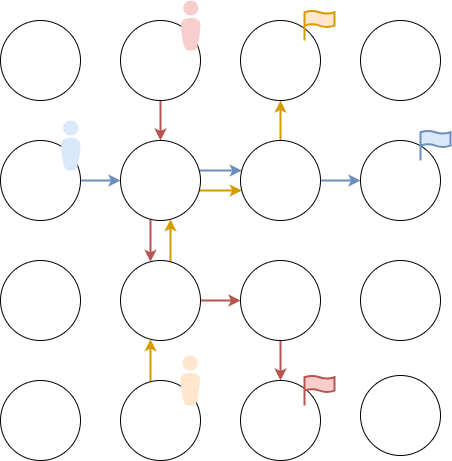
\includegraphics[width=6cm]{img/partial_solving_example.png}
\end{figure}
\end{frame}


\subsection{Pre-computed paths}
\begin{frame}[fragile]{An example using pre-computed paths}
    \begin{figure}[H]
    \centering
    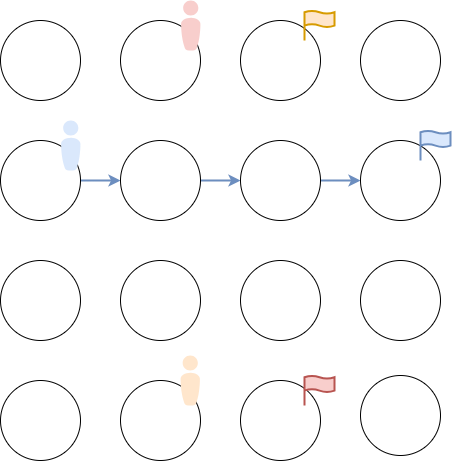
\includegraphics[width=5.5cm]{img/pre_computed_path_solving.drawio.png}
\end{figure}
\end{frame}


\subsection{Subgraph}
\begin{frame}[fragile]{An example using subgraph}
    \begin{figure}[H]
        \centering
        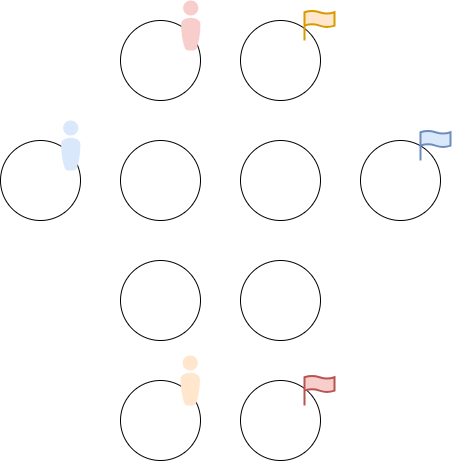
\includegraphics[width=6cm]{img/subgraph_solving.png}
    \end{figure}
\end{frame}

\begin{frame}[fragile]{Subgraph extention strategies}
    
    \begin{figure}[H]
        \centering
        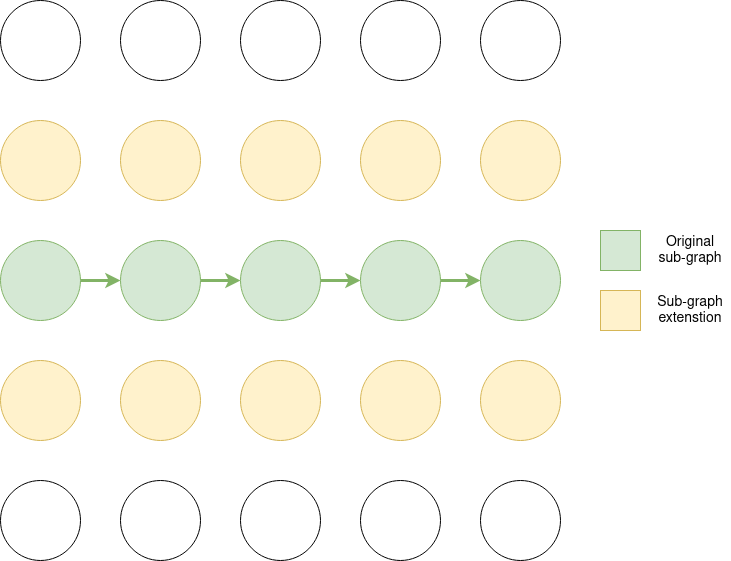
\includegraphics[width=\widthimg]{img/corridor.drawio.png}
    \end{figure}
\end{frame}

\begin{frame}[fragile]{Subgraph extention strategies}
    \begin{figure}[H]
        \centering
        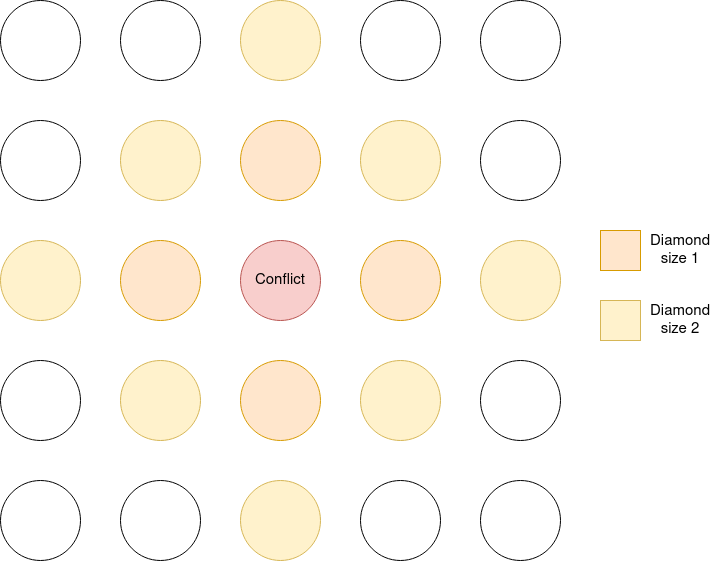
\includegraphics[width=\widthimg]{img/diamond.drawio.png}
      \end{figure}
      
\end{frame}